\section{Results \& analysis}
\begin{figure}[h]
  \centering
  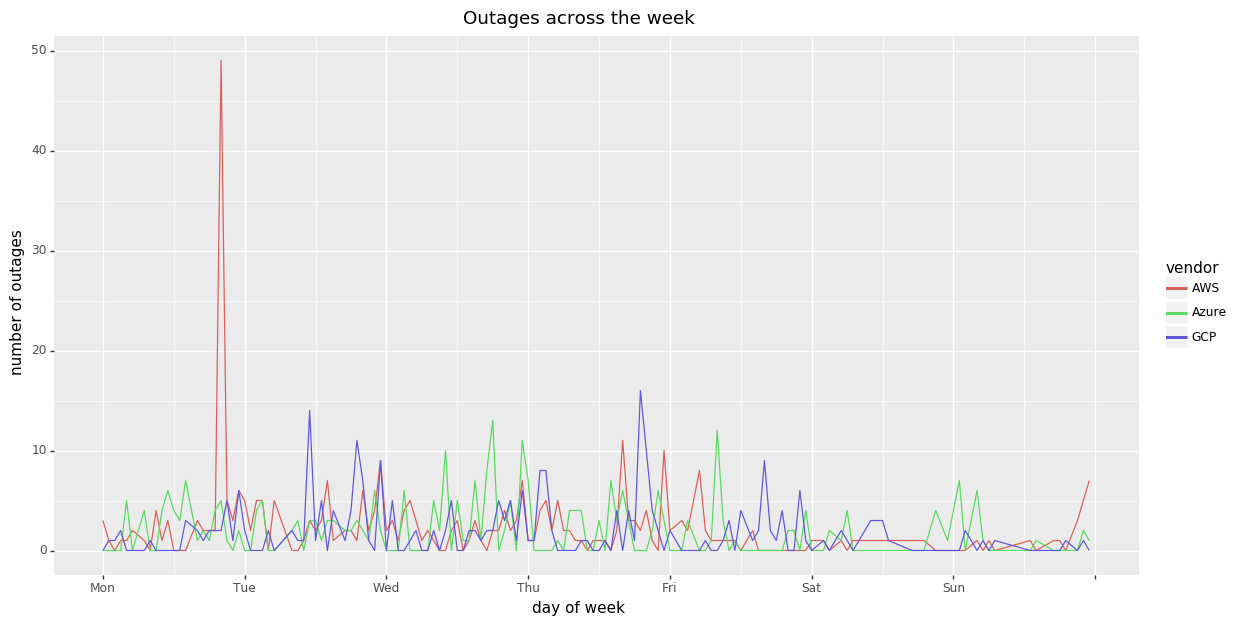
\includegraphics[scale=0.5]{outages-across-week.png}
  \caption{Distribution of outages across the week, by vendor.}
  \label{fig:outages across week}
\end{figure}

We first observe the distribution of outages across the week, this is shown in \autoref{fig:outages across week}.
GCP and AWS both show significant peaks at two points during the week: around the middle (Tuesday and Wednesday), and at the start of the weekend (Friday and Saturday).
AWS also shows an increase in outages in the afternoon/evening hours on Sunday.
The data provided by Azure does not indicate any clear trends.

\begin{figure}[h]
  \centering
  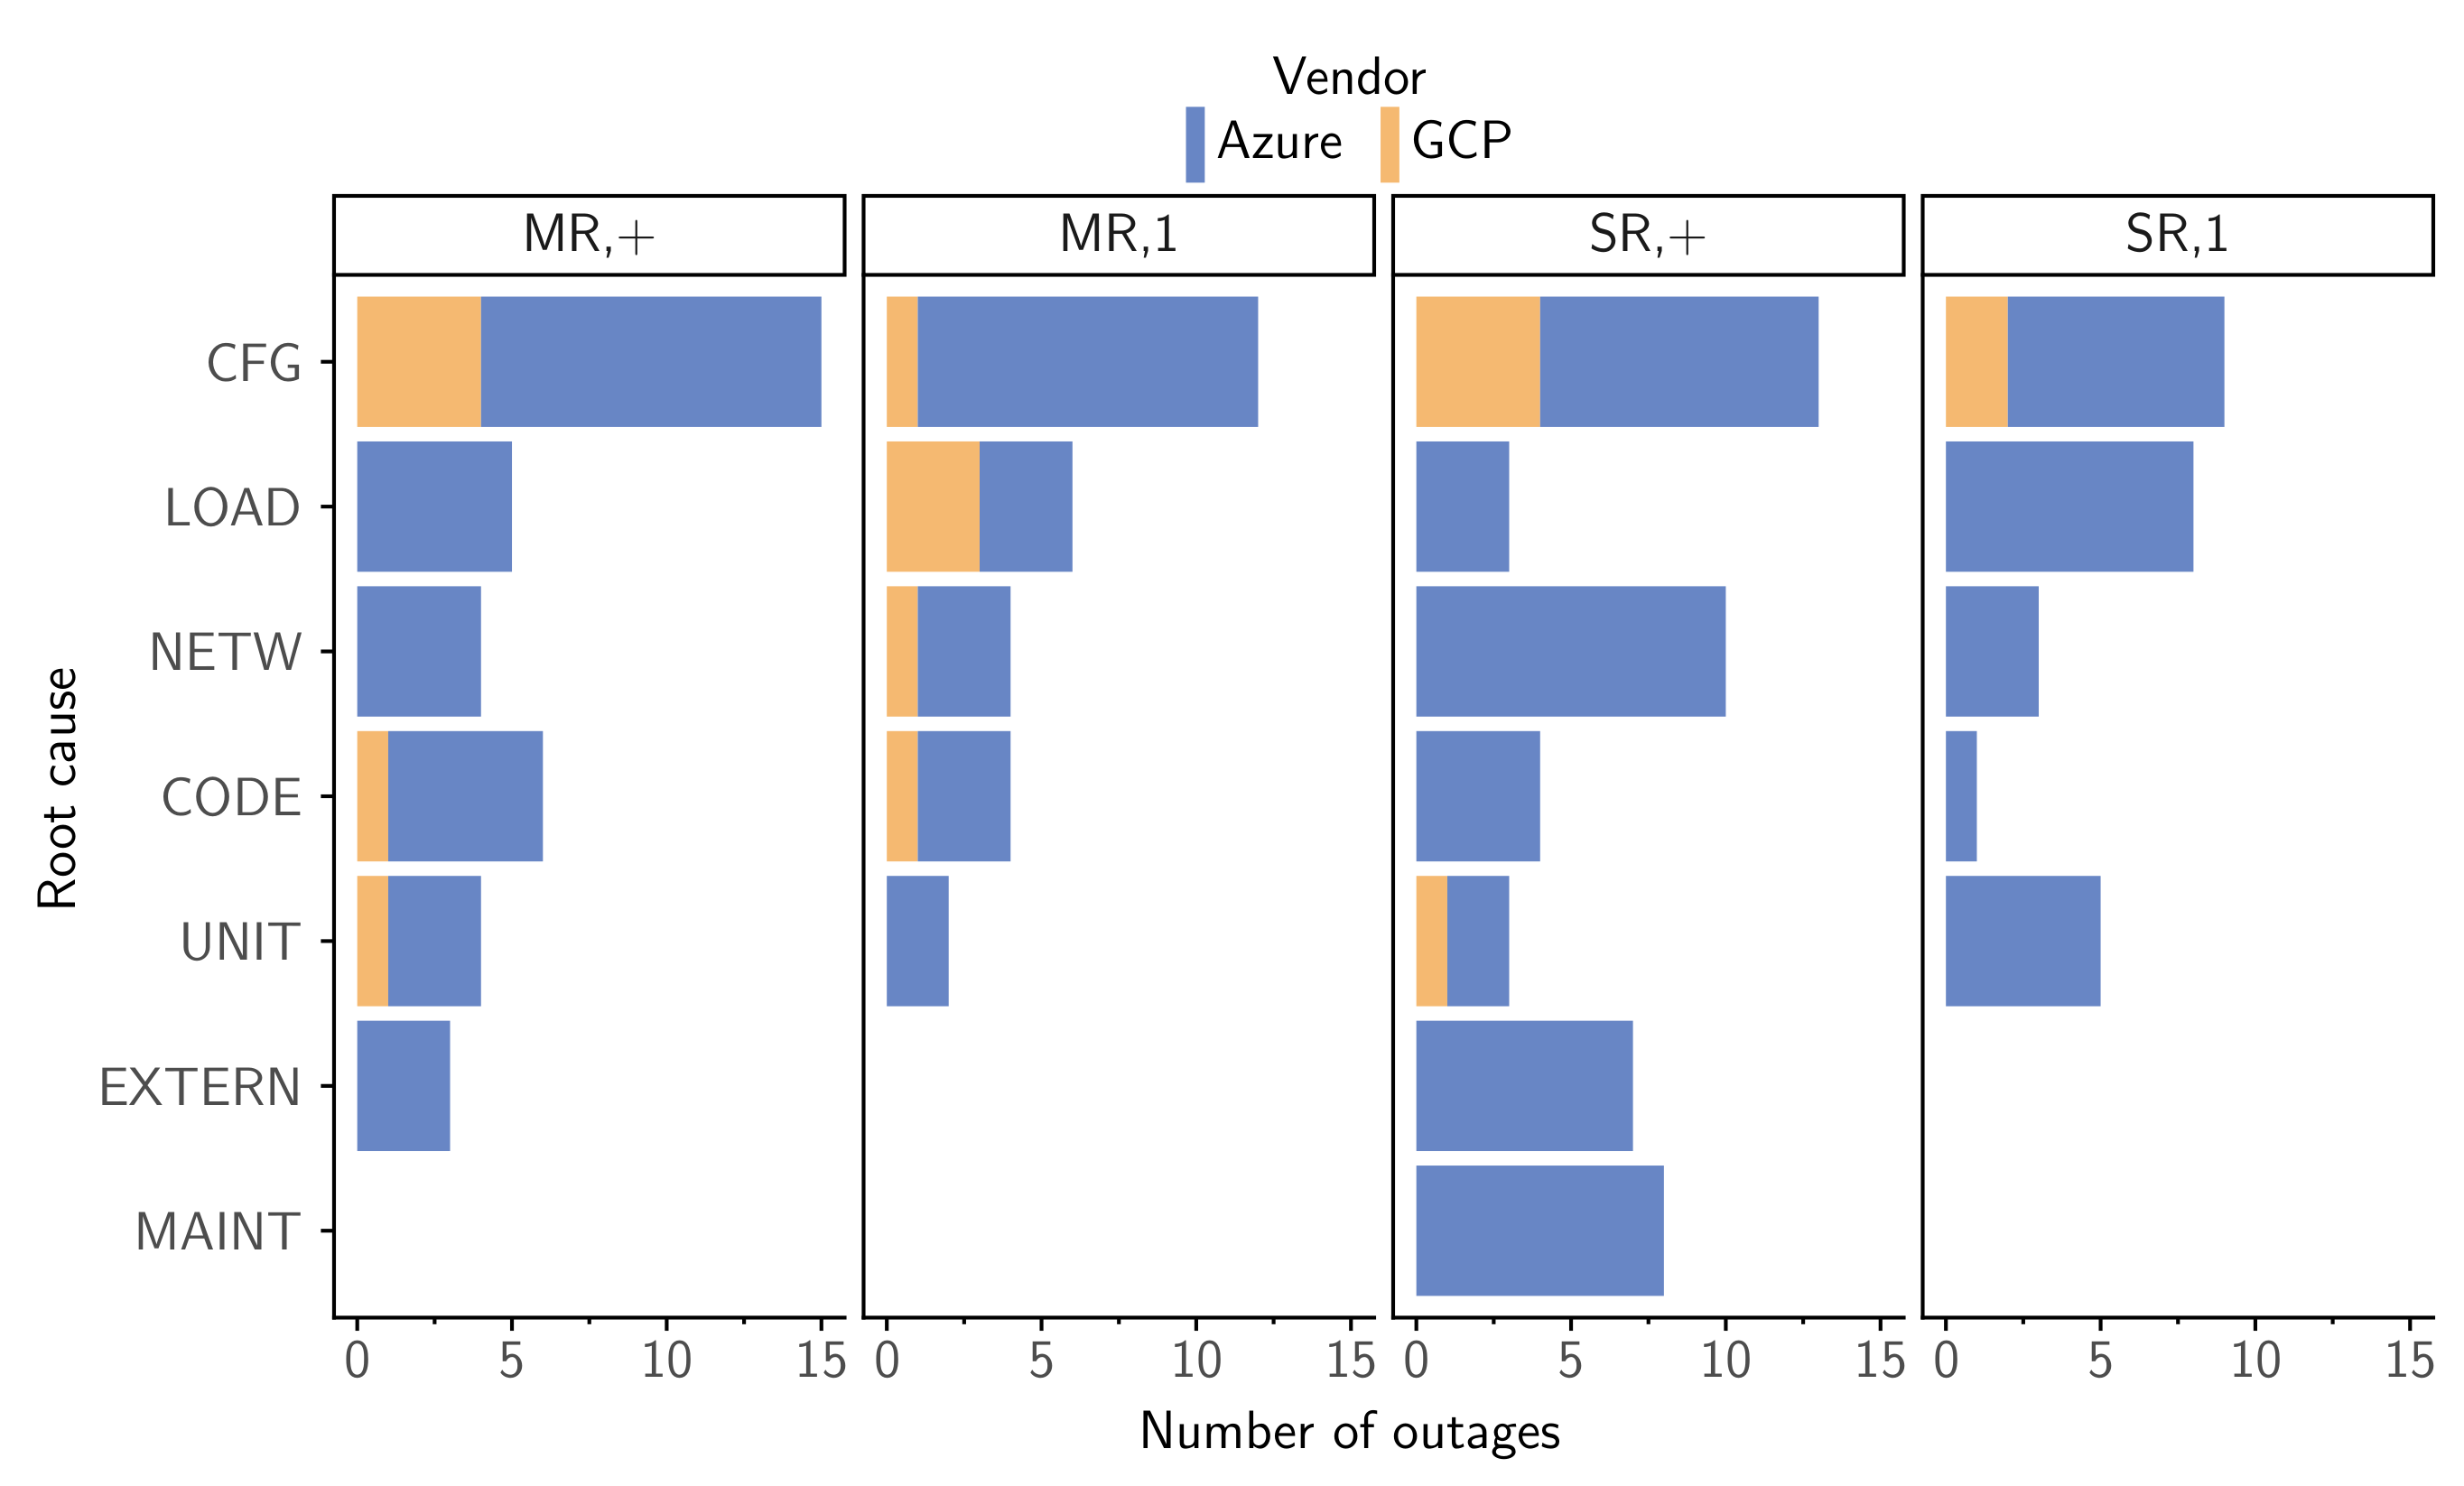
\includegraphics[scale=0.5]{root-causes-by-severity.png}
  \caption{Root causes of outages across varying severity levels, by vendor. (MR = multiple regions, SR = single region, 1 = one service, + = multiple services)}
  \label{fig:root causes by severity}
\end{figure}

We next analyse the distribution of outages across root causes and severity levels.
We identify seven classes of root causes: UNIT (individual nodes or instances), NETW (related to the internal or external network), MAINT (side effects caused by maintenance), LOAD (increased load on the service), EXTERN (external causes, i.e. environmental or third-party), CODE (code errors/bugs), and CFG (configuration errors).
We further separate the outages by vendor, indicated by the color of the bar in \autoref{fig:root causes by severity}.
Excluded from the plot are outages that did not provide a root cause (a total of \result{np-root-causes-by-severity-cause}), a range (\result{np-root-causes-by-severity-range}), or the number of affected services (\result{np-root-causes-by-severity-services}).
AWS also has a third range category, the `single availability zone', which is narrower than a single region. % TODO: maybe put this in method?
However, as this is only applicable to AWS services, this category was merged with `single region'.

The majority of outages across all levels of severity are caused by configuration errors.
For multi-regional outages, the configuration category accounts for the majority by a wide margin.
On the other hand, for single-region outages, there are multiple leading causes: apart from configuration errors, outages affecting one service are also caused by increased load and failing instances, and those affecting more than one service are also caused by network errors and maintenance side effects.
All AWS outages that specified a root cause were caused by external events; however, it is important to note here that 97.9\% of AWS outages did not specify a cause, so this finding is limited due to a lack of data.

\begin{figure}[h]
  \centering
  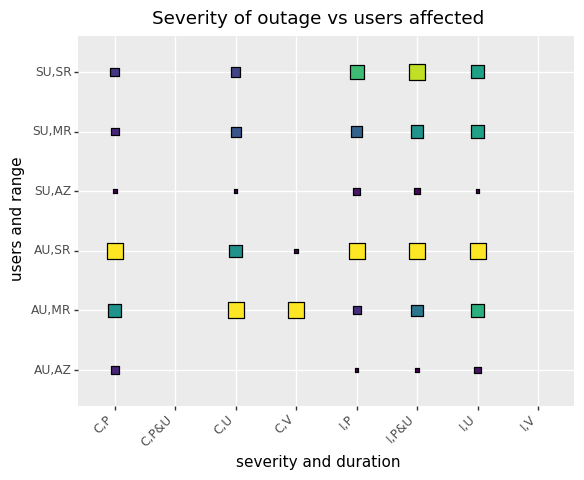
\includegraphics[scale=0.5]{severity-vs-users-affected.png}
  \caption{Severity of an outage and the users affected by the outage. (SU = some users, AU = all users, C = continuous, I = intermittent, P = performance degradation, U = unavailable, V = visual)}
  \label{fig:severity vs users}
\end{figure}

Next, we consider the users affected in an outage, depending on its severity.
We exclude events that did not state the affected users (\result{np-severity-vs-users-affected-users}), area (\result{np-severity-vs-users-affected-severity}), severity (\result{np-severity-vs-users-affected-severity}), or duration (\result{np-severity-vs-users-affected-duration}).
The first immediate finding from \autoref{fig:severity vs users} is that the majority of outages result in one or more services becoming intermittently unavailable.
For outages affecting all users, in a single region or in multiple regions, there is a higher proportion of outages that cause a service to be intermittently degraded or unavailable than for outages affecting some users.
Furthermore, the majority of outages that resulted in a service being continuously unavailable (for some period of time) affected all users in multiple regions.
When the performance of one or more services is degraded, it generally happens for a continuous period of time.

\begin{figure}[h]
  \centering
  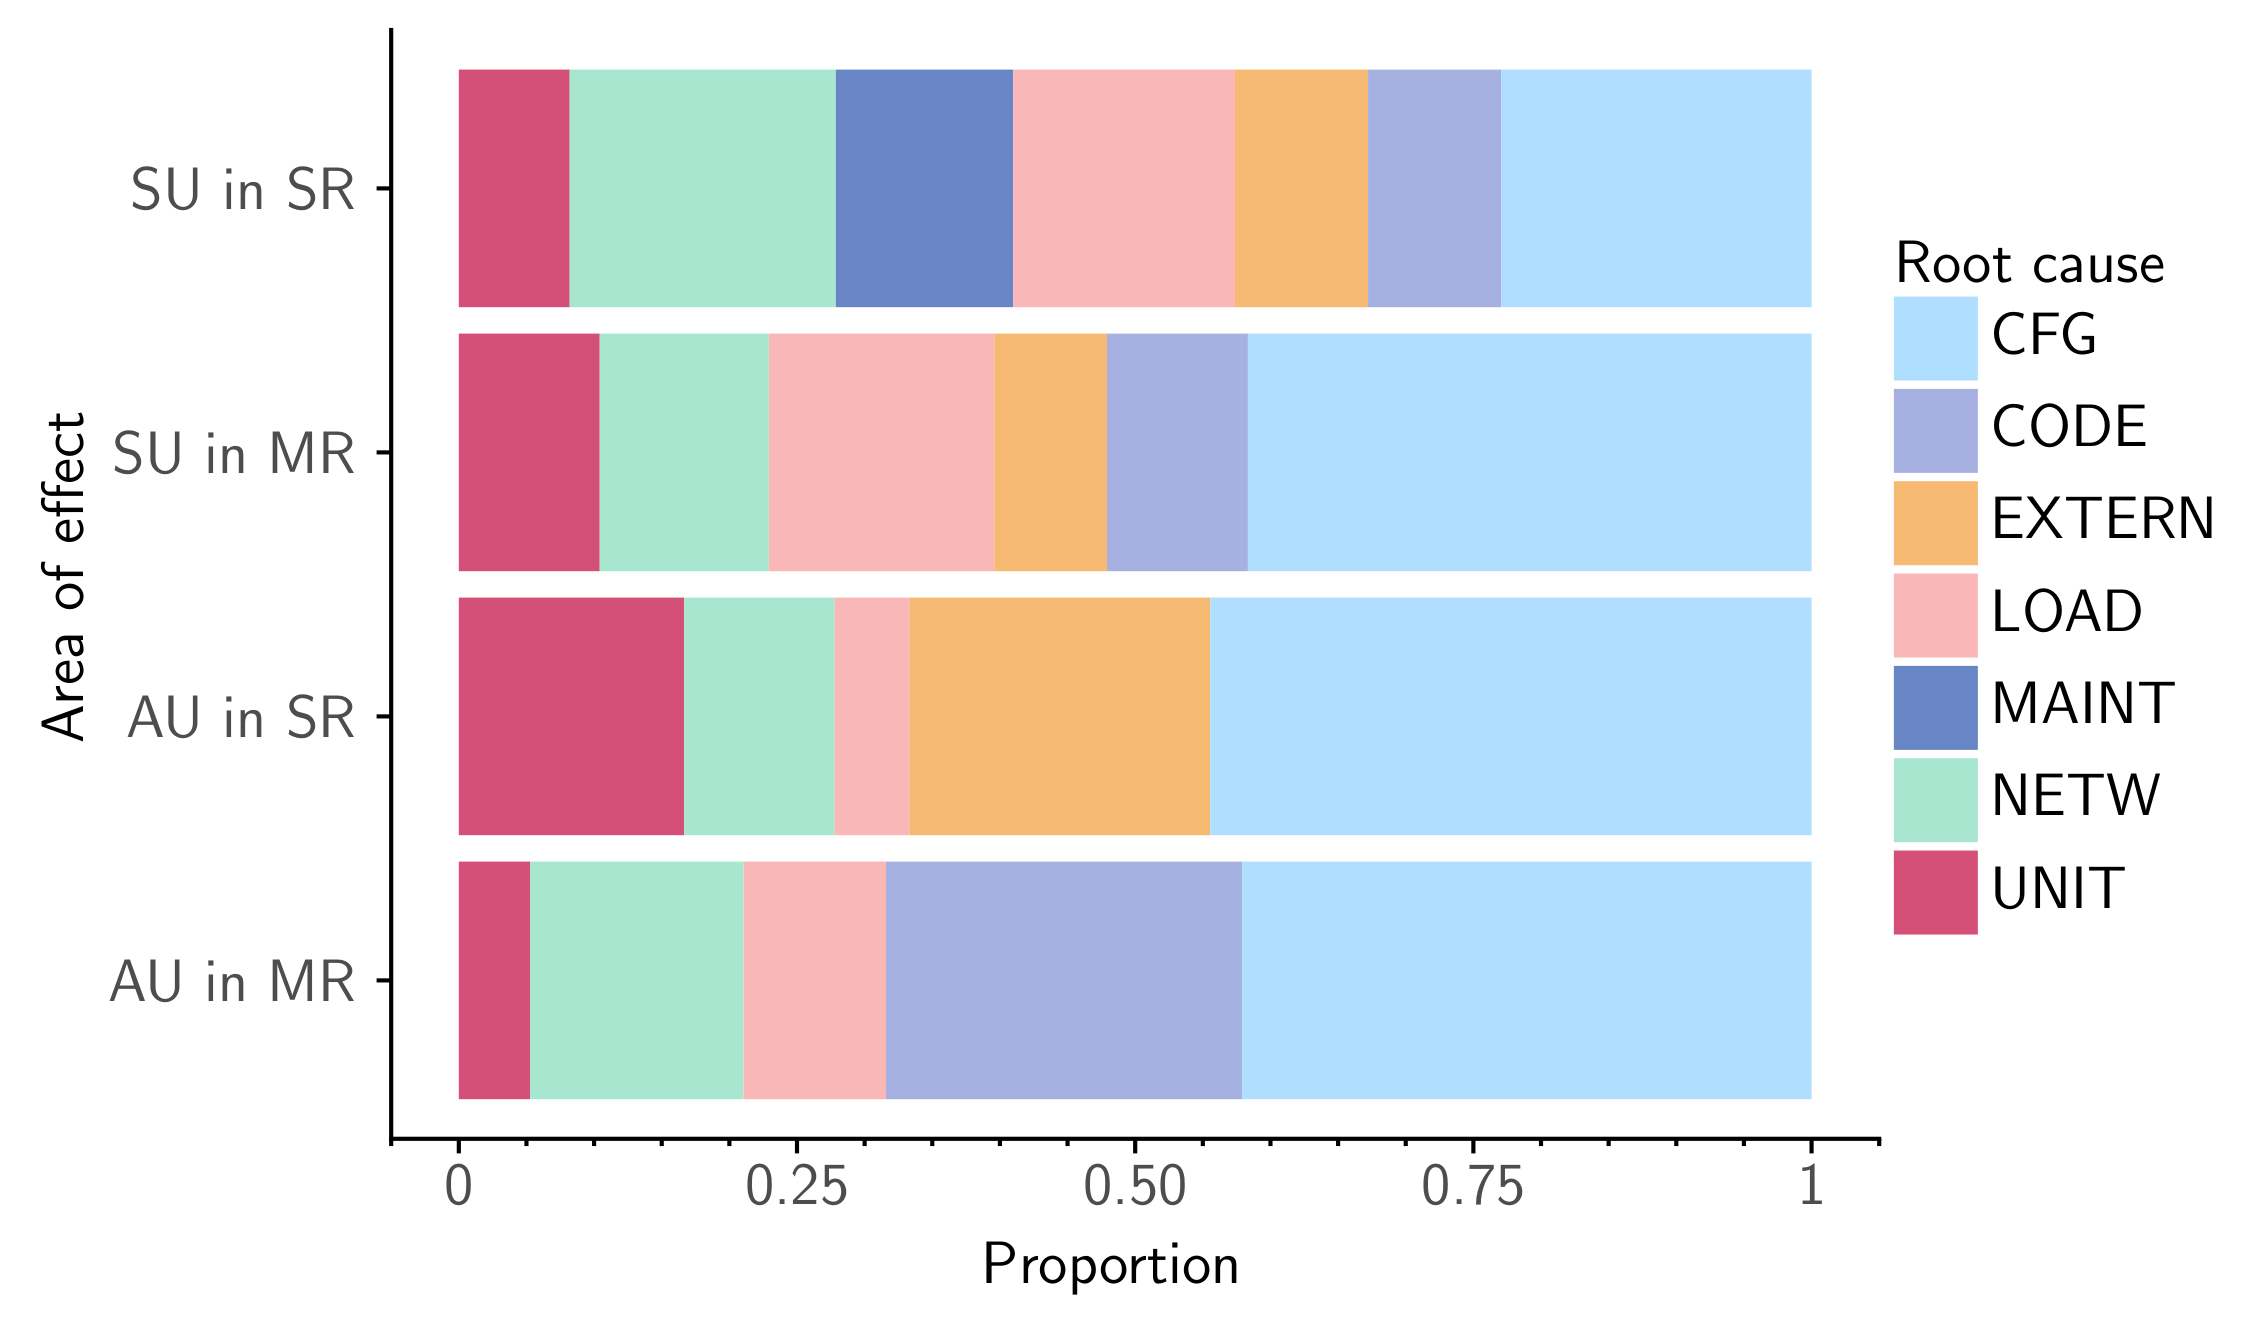
\includegraphics[scale=0.5]{range-users-vs-root-cause.png}
  \caption{Root causes of outages at various impact ranges. (SU = some users, AU = all users, SR = single region, MR = multiple regions)}
  \label{fig:causes vs impact ranges}
\end{figure}

We also analyze the root causes of outages, separated by the range of the outage.
We define the range of an outage as the affected users (all or some) and the impacted area (single region or multiple regions).
Here we exclude those events that did not provide a cause (\result{np-range-users-vs-root-cause-cause}), an area of effect (\result{np-range-users-vs-root-cause-range}), or the affected users (\result{np-range-users-vs-root-cause-users}).
From \autoref{fig:causes vs impact ranges}, we conclude that configuration errors account for the majority of outages with the widest impact range (all users in multiple regions).
The second main cause of such outages are code errors, which interestingly do not play a major role in single-region outages, and do not appear as a cause of single-region outages affecting all users.
Failing instances are mainly a cause of single-region outages, more so for outages that affect all users -- this is probably due to the fact that individual instances, nodes, or clusters are more localised. % TODO: requires citation
From the available data, it seems that outages caused as a maintenance side effect only affect some users of the service, mostly in a single region.
The majority of outages caused by network issues affect some users in a single region, though they also play a somewhat significant role in the other range categories (accounting for around 10\% of the outages in each range category).

\begin{figure}[h]
  \centering
  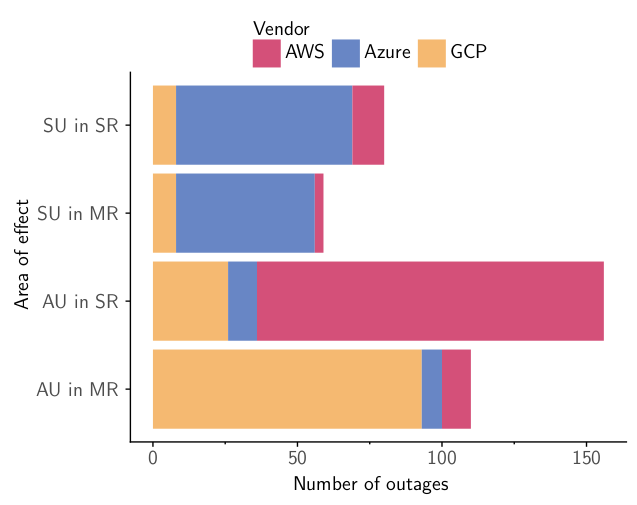
\includegraphics[scale=0.5]{users-affected-by-vendor.png}
  \caption{Range of outages by vendor. (AU = all users, SU = some users, SR = single region, MR = multiple regions)}
  \label{fig:range by vendor}
\end{figure}

We continue with the definition of range as the affected users and the area of effect, and analyse the distribution of outages per vendor, in figure \autoref{fig:range by vendor}.
We do not include events that are missing information about the users (\result{np-users-affected-by-vendor-users}) or the area of effect (\result{np-users-affected-by-vendor-range}).
We observe that the range of the majority of outages depends on the vendor.
The majority of GCP outages affect all users in multiple regions, while the majority of AWS outages affect all users in a single region.
For Azure services, the outages mostly affect some users, with an approximately equal distribution between a single region and multiple regions.

